% Created by tikzDevice version 0.7.0 on 2015-07-02 12:23:01
% !TEX encoding = UTF-8 Unicode
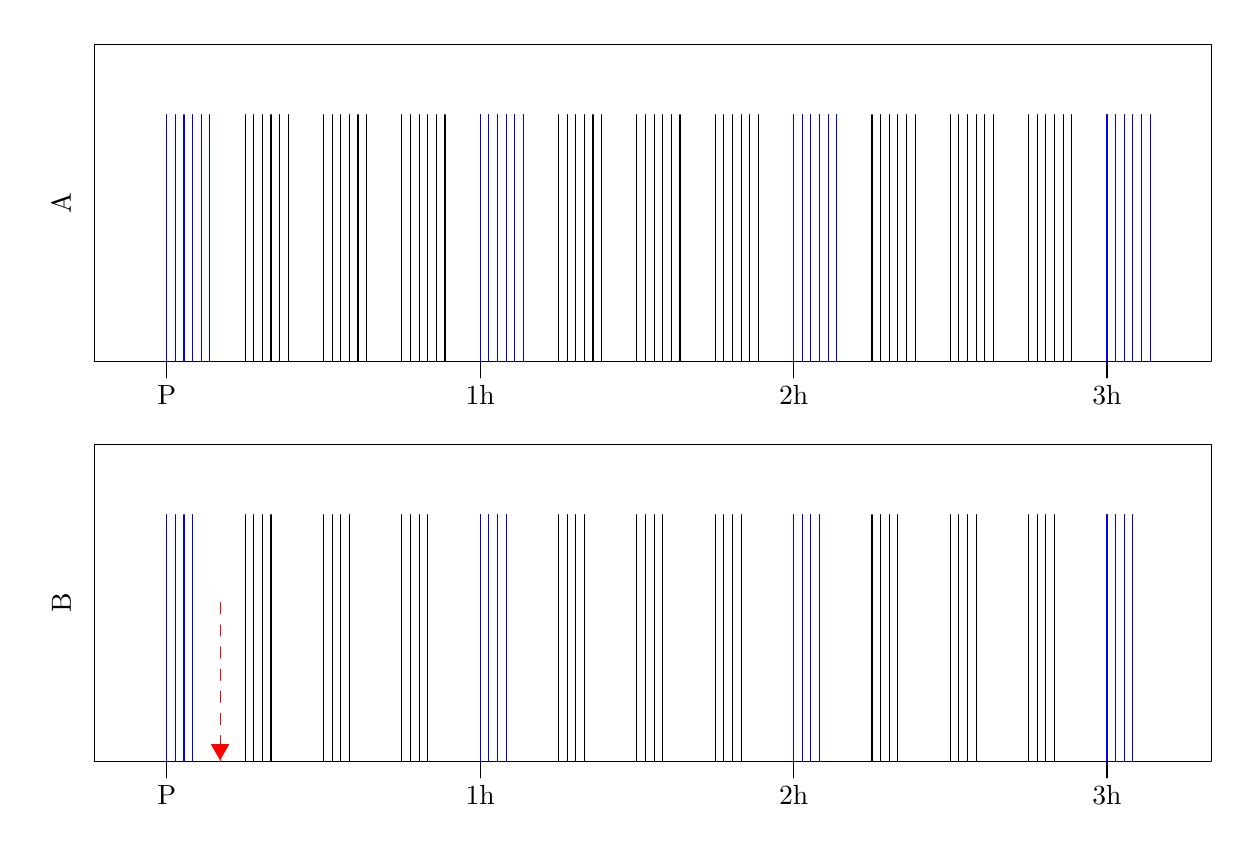
\begin{tikzpicture}[x=1pt,y=1pt]
\definecolor[named]{fillColor}{rgb}{1.00,1.00,1.00}
\path[use as bounding box,fill=fillColor,fill opacity=0.00] (0,0) rectangle (433.62,289.08);
\begin{scope}
\path[clip] (  0.00,  0.00) rectangle (433.62,289.08);
\definecolor[named]{drawColor}{rgb}{0.00,0.00,0.00}

\path[draw=drawColor,line width= 0.4pt,line join=round,line cap=round] ( 24.00,168.54) --
	(427.62,168.54) --
	(427.62,283.08) --
	( 24.00,283.08) --
	( 24.00,168.54);
\end{scope}
\begin{scope}
\path[clip] (  0.00,144.54) rectangle (433.62,289.08);
\definecolor[named]{drawColor}{rgb}{0.00,0.00,0.00}

\node[text=drawColor,rotate= 90.00,anchor=base,inner sep=0pt, outer sep=0pt, scale=  1.00] at ( 15.60,225.81) {A};
\end{scope}
\begin{scope}
\path[clip] (  0.00,  0.00) rectangle (433.62,289.08);
\definecolor[named]{drawColor}{rgb}{0.00,0.00,0.00}

\path[draw=drawColor,line width= 0.4pt,line join=round,line cap=round] ( 50.27,168.54) -- (390.02,168.54);

\path[draw=drawColor,line width= 0.4pt,line join=round,line cap=round] ( 50.27,168.54) -- ( 50.27,162.54);

\path[draw=drawColor,line width= 0.4pt,line join=round,line cap=round] (163.52,168.54) -- (163.52,162.54);

\path[draw=drawColor,line width= 0.4pt,line join=round,line cap=round] (276.77,168.54) -- (276.77,162.54);

\path[draw=drawColor,line width= 0.4pt,line join=round,line cap=round] (390.02,168.54) -- (390.02,162.54);

\node[text=drawColor,anchor=base,inner sep=0pt, outer sep=0pt, scale=  1.00] at ( 50.27,152.94) {P};

\node[text=drawColor,anchor=base,inner sep=0pt, outer sep=0pt, scale=  1.00] at (163.52,152.94) {1h};

\node[text=drawColor,anchor=base,inner sep=0pt, outer sep=0pt, scale=  1.00] at (276.77,152.94) {2h};

\node[text=drawColor,anchor=base,inner sep=0pt, outer sep=0pt, scale=  1.00] at (390.02,152.94) {3h};
\end{scope}
\begin{scope}
\path[clip] ( 24.00,168.54) rectangle (427.62,283.08);
\definecolor[named]{drawColor}{rgb}{0.00,0.00,1.00}

\path[draw=drawColor,line width= 0.4pt,line join=round,line cap=round] ( 50.27, 66.73) -- ( 50.27,257.63);

\path[draw=drawColor,line width= 0.4pt,line join=round,line cap=round] ( 53.39, 66.73) -- ( 53.39,257.63);

\path[draw=drawColor,line width= 0.4pt,line join=round,line cap=round] ( 56.50, 66.73) -- ( 56.50,257.63);

\path[draw=drawColor,line width= 0.4pt,line join=round,line cap=round] ( 59.62, 66.73) -- ( 59.62,257.63);

\path[draw=drawColor,line width= 0.4pt,line join=round,line cap=round] ( 62.73, 66.73) -- ( 62.73,257.63);

\path[draw=drawColor,line width= 0.4pt,line join=round,line cap=round] ( 65.85, 66.73) -- ( 65.85,257.63);
\definecolor[named]{drawColor}{rgb}{0.00,0.00,0.00}

\path[draw=drawColor,line width= 0.4pt,line join=round,line cap=round] ( 78.59, 66.73) -- ( 78.59,257.63);

\path[draw=drawColor,line width= 0.4pt,line join=round,line cap=round] ( 81.70, 66.73) -- ( 81.70,257.63);

\path[draw=drawColor,line width= 0.4pt,line join=round,line cap=round] ( 84.81, 66.73) -- ( 84.81,257.63);

\path[draw=drawColor,line width= 0.4pt,line join=round,line cap=round] ( 87.93, 66.73) -- ( 87.93,257.63);

\path[draw=drawColor,line width= 0.4pt,line join=round,line cap=round] ( 91.04, 66.73) -- ( 91.04,257.63);

\path[draw=drawColor,line width= 0.4pt,line join=round,line cap=round] ( 94.16, 66.73) -- ( 94.16,257.63);

\path[draw=drawColor,line width= 0.4pt,line join=round,line cap=round] (106.90, 66.73) -- (106.90,257.63);

\path[draw=drawColor,line width= 0.4pt,line join=round,line cap=round] (110.01, 66.73) -- (110.01,257.63);

\path[draw=drawColor,line width= 0.4pt,line join=round,line cap=round] (113.13, 66.73) -- (113.13,257.63);

\path[draw=drawColor,line width= 0.4pt,line join=round,line cap=round] (116.24, 66.73) -- (116.24,257.63);

\path[draw=drawColor,line width= 0.4pt,line join=round,line cap=round] (119.36, 66.73) -- (119.36,257.63);

\path[draw=drawColor,line width= 0.4pt,line join=round,line cap=round] (122.47, 66.73) -- (122.47,257.63);

\path[draw=drawColor,line width= 0.4pt,line join=round,line cap=round] (135.21, 66.73) -- (135.21,257.63);

\path[draw=drawColor,line width= 0.4pt,line join=round,line cap=round] (138.33, 66.73) -- (138.33,257.63);

\path[draw=drawColor,line width= 0.4pt,line join=round,line cap=round] (141.44, 66.73) -- (141.44,257.63);

\path[draw=drawColor,line width= 0.4pt,line join=round,line cap=round] (144.55, 66.73) -- (144.55,257.63);

\path[draw=drawColor,line width= 0.4pt,line join=round,line cap=round] (147.67, 66.73) -- (147.67,257.63);

\path[draw=drawColor,line width= 0.4pt,line join=round,line cap=round] (150.78, 66.73) -- (150.78,257.63);

\path[draw=drawColor,line width= 0.4pt,line join=round,line cap=round] (163.52, 66.73) -- (163.52,257.63);

\path[draw=drawColor,line width= 0.4pt,line join=round,line cap=round] (166.64, 66.73) -- (166.64,257.63);

\path[draw=drawColor,line width= 0.4pt,line join=round,line cap=round] (169.75, 66.73) -- (169.75,257.63);

\path[draw=drawColor,line width= 0.4pt,line join=round,line cap=round] (172.87, 66.73) -- (172.87,257.63);

\path[draw=drawColor,line width= 0.4pt,line join=round,line cap=round] (175.98, 66.73) -- (175.98,257.63);

\path[draw=drawColor,line width= 0.4pt,line join=round,line cap=round] (179.09, 66.73) -- (179.09,257.63);
\definecolor[named]{drawColor}{rgb}{0.00,0.00,1.00}

\path[draw=drawColor,line width= 0.4pt,line join=round,line cap=round] (163.52, 66.73) -- (163.52,257.63);

\path[draw=drawColor,line width= 0.4pt,line join=round,line cap=round] (166.64, 66.73) -- (166.64,257.63);

\path[draw=drawColor,line width= 0.4pt,line join=round,line cap=round] (169.75, 66.73) -- (169.75,257.63);

\path[draw=drawColor,line width= 0.4pt,line join=round,line cap=round] (172.87, 66.73) -- (172.87,257.63);

\path[draw=drawColor,line width= 0.4pt,line join=round,line cap=round] (175.98, 66.73) -- (175.98,257.63);

\path[draw=drawColor,line width= 0.4pt,line join=round,line cap=round] (179.09, 66.73) -- (179.09,257.63);
\definecolor[named]{drawColor}{rgb}{0.00,0.00,0.00}

\path[draw=drawColor,line width= 0.4pt,line join=round,line cap=round] (191.84, 66.73) -- (191.84,257.63);

\path[draw=drawColor,line width= 0.4pt,line join=round,line cap=round] (194.95, 66.73) -- (194.95,257.63);

\path[draw=drawColor,line width= 0.4pt,line join=round,line cap=round] (198.06, 66.73) -- (198.06,257.63);

\path[draw=drawColor,line width= 0.4pt,line join=round,line cap=round] (201.18, 66.73) -- (201.18,257.63);

\path[draw=drawColor,line width= 0.4pt,line join=round,line cap=round] (204.29, 66.73) -- (204.29,257.63);

\path[draw=drawColor,line width= 0.4pt,line join=round,line cap=round] (207.41, 66.73) -- (207.41,257.63);

\path[draw=drawColor,line width= 0.4pt,line join=round,line cap=round] (220.15, 66.73) -- (220.15,257.63);

\path[draw=drawColor,line width= 0.4pt,line join=round,line cap=round] (223.26, 66.73) -- (223.26,257.63);

\path[draw=drawColor,line width= 0.4pt,line join=round,line cap=round] (226.38, 66.73) -- (226.38,257.63);

\path[draw=drawColor,line width= 0.4pt,line join=round,line cap=round] (229.49, 66.73) -- (229.49,257.63);

\path[draw=drawColor,line width= 0.4pt,line join=round,line cap=round] (232.60, 66.73) -- (232.60,257.63);

\path[draw=drawColor,line width= 0.4pt,line join=round,line cap=round] (235.72, 66.73) -- (235.72,257.63);

\path[draw=drawColor,line width= 0.4pt,line join=round,line cap=round] (248.46, 66.73) -- (248.46,257.63);

\path[draw=drawColor,line width= 0.4pt,line join=round,line cap=round] (251.57, 66.73) -- (251.57,257.63);

\path[draw=drawColor,line width= 0.4pt,line join=round,line cap=round] (254.69, 66.73) -- (254.69,257.63);

\path[draw=drawColor,line width= 0.4pt,line join=round,line cap=round] (257.80, 66.73) -- (257.80,257.63);

\path[draw=drawColor,line width= 0.4pt,line join=round,line cap=round] (260.92, 66.73) -- (260.92,257.63);

\path[draw=drawColor,line width= 0.4pt,line join=round,line cap=round] (264.03, 66.73) -- (264.03,257.63);

\path[draw=drawColor,line width= 0.4pt,line join=round,line cap=round] (276.77, 66.73) -- (276.77,257.63);

\path[draw=drawColor,line width= 0.4pt,line join=round,line cap=round] (279.89, 66.73) -- (279.89,257.63);

\path[draw=drawColor,line width= 0.4pt,line join=round,line cap=round] (283.00, 66.73) -- (283.00,257.63);

\path[draw=drawColor,line width= 0.4pt,line join=round,line cap=round] (286.12, 66.73) -- (286.12,257.63);

\path[draw=drawColor,line width= 0.4pt,line join=round,line cap=round] (289.23, 66.73) -- (289.23,257.63);

\path[draw=drawColor,line width= 0.4pt,line join=round,line cap=round] (292.34, 66.73) -- (292.34,257.63);
\definecolor[named]{drawColor}{rgb}{0.00,0.00,1.00}

\path[draw=drawColor,line width= 0.4pt,line join=round,line cap=round] (276.77, 66.73) -- (276.77,257.63);

\path[draw=drawColor,line width= 0.4pt,line join=round,line cap=round] (279.89, 66.73) -- (279.89,257.63);

\path[draw=drawColor,line width= 0.4pt,line join=round,line cap=round] (283.00, 66.73) -- (283.00,257.63);

\path[draw=drawColor,line width= 0.4pt,line join=round,line cap=round] (286.12, 66.73) -- (286.12,257.63);

\path[draw=drawColor,line width= 0.4pt,line join=round,line cap=round] (289.23, 66.73) -- (289.23,257.63);

\path[draw=drawColor,line width= 0.4pt,line join=round,line cap=round] (292.34, 66.73) -- (292.34,257.63);
\definecolor[named]{drawColor}{rgb}{0.00,0.00,0.00}

\path[draw=drawColor,line width= 0.4pt,line join=round,line cap=round] (305.08, 66.73) -- (305.08,257.63);

\path[draw=drawColor,line width= 0.4pt,line join=round,line cap=round] (308.20, 66.73) -- (308.20,257.63);

\path[draw=drawColor,line width= 0.4pt,line join=round,line cap=round] (311.31, 66.73) -- (311.31,257.63);

\path[draw=drawColor,line width= 0.4pt,line join=round,line cap=round] (314.43, 66.73) -- (314.43,257.63);

\path[draw=drawColor,line width= 0.4pt,line join=round,line cap=round] (317.54, 66.73) -- (317.54,257.63);

\path[draw=drawColor,line width= 0.4pt,line join=round,line cap=round] (320.66, 66.73) -- (320.66,257.63);

\path[draw=drawColor,line width= 0.4pt,line join=round,line cap=round] (333.40, 66.73) -- (333.40,257.63);

\path[draw=drawColor,line width= 0.4pt,line join=round,line cap=round] (336.51, 66.73) -- (336.51,257.63);

\path[draw=drawColor,line width= 0.4pt,line join=round,line cap=round] (339.63, 66.73) -- (339.63,257.63);

\path[draw=drawColor,line width= 0.4pt,line join=round,line cap=round] (342.74, 66.73) -- (342.74,257.63);

\path[draw=drawColor,line width= 0.4pt,line join=round,line cap=round] (345.85, 66.73) -- (345.85,257.63);

\path[draw=drawColor,line width= 0.4pt,line join=round,line cap=round] (348.97, 66.73) -- (348.97,257.63);

\path[draw=drawColor,line width= 0.4pt,line join=round,line cap=round] (361.71, 66.73) -- (361.71,257.63);

\path[draw=drawColor,line width= 0.4pt,line join=round,line cap=round] (364.82, 66.73) -- (364.82,257.63);

\path[draw=drawColor,line width= 0.4pt,line join=round,line cap=round] (367.94, 66.73) -- (367.94,257.63);

\path[draw=drawColor,line width= 0.4pt,line join=round,line cap=round] (371.05, 66.73) -- (371.05,257.63);

\path[draw=drawColor,line width= 0.4pt,line join=round,line cap=round] (374.17, 66.73) -- (374.17,257.63);

\path[draw=drawColor,line width= 0.4pt,line join=round,line cap=round] (377.28, 66.73) -- (377.28,257.63);

\path[draw=drawColor,line width= 0.4pt,line join=round,line cap=round] (390.02, 66.73) -- (390.02,257.63);

\path[draw=drawColor,line width= 0.4pt,line join=round,line cap=round] (393.14, 66.73) -- (393.14,257.63);

\path[draw=drawColor,line width= 0.4pt,line join=round,line cap=round] (396.25, 66.73) -- (396.25,257.63);

\path[draw=drawColor,line width= 0.4pt,line join=round,line cap=round] (399.36, 66.73) -- (399.36,257.63);

\path[draw=drawColor,line width= 0.4pt,line join=round,line cap=round] (402.48, 66.73) -- (402.48,257.63);

\path[draw=drawColor,line width= 0.4pt,line join=round,line cap=round] (405.59, 66.73) -- (405.59,257.63);
\definecolor[named]{drawColor}{rgb}{0.00,0.00,1.00}

\path[draw=drawColor,line width= 0.4pt,line join=round,line cap=round] (390.02, 66.73) -- (390.02,257.63);

\path[draw=drawColor,line width= 0.4pt,line join=round,line cap=round] (393.14, 66.73) -- (393.14,257.63);

\path[draw=drawColor,line width= 0.4pt,line join=round,line cap=round] (396.25, 66.73) -- (396.25,257.63);

\path[draw=drawColor,line width= 0.4pt,line join=round,line cap=round] (399.36, 66.73) -- (399.36,257.63);

\path[draw=drawColor,line width= 0.4pt,line join=round,line cap=round] (402.48, 66.73) -- (402.48,257.63);

\path[draw=drawColor,line width= 0.4pt,line join=round,line cap=round] (405.59, 66.73) -- (405.59,257.63);
\end{scope}
\begin{scope}
\path[clip] (  0.00,  0.00) rectangle (433.62,289.08);
\definecolor[named]{drawColor}{rgb}{0.00,0.00,0.00}

\path[draw=drawColor,line width= 0.4pt,line join=round,line cap=round] ( 24.00, 24.00) --
	(427.62, 24.00) --
	(427.62,138.54) --
	( 24.00,138.54) --
	( 24.00, 24.00);
\end{scope}
\begin{scope}
\path[clip] (  0.00,  0.00) rectangle (433.62,144.54);
\definecolor[named]{drawColor}{rgb}{0.00,0.00,0.00}

\node[text=drawColor,rotate= 90.00,anchor=base,inner sep=0pt, outer sep=0pt, scale=  1.00] at ( 15.60, 81.27) {B};
\end{scope}
\begin{scope}
\path[clip] (  0.00,  0.00) rectangle (433.62,289.08);
\definecolor[named]{drawColor}{rgb}{0.00,0.00,0.00}

\path[draw=drawColor,line width= 0.4pt,line join=round,line cap=round] ( 50.27, 24.00) -- (390.02, 24.00);

\path[draw=drawColor,line width= 0.4pt,line join=round,line cap=round] ( 50.27, 24.00) -- ( 50.27, 18.00);

\path[draw=drawColor,line width= 0.4pt,line join=round,line cap=round] (163.52, 24.00) -- (163.52, 18.00);

\path[draw=drawColor,line width= 0.4pt,line join=round,line cap=round] (276.77, 24.00) -- (276.77, 18.00);

\path[draw=drawColor,line width= 0.4pt,line join=round,line cap=round] (390.02, 24.00) -- (390.02, 18.00);

\node[text=drawColor,anchor=base,inner sep=0pt, outer sep=0pt, scale=  1.00] at ( 50.27,  8.40) {P};

\node[text=drawColor,anchor=base,inner sep=0pt, outer sep=0pt, scale=  1.00] at (163.52,  8.40) {1h};

\node[text=drawColor,anchor=base,inner sep=0pt, outer sep=0pt, scale=  1.00] at (276.77,  8.40) {2h};

\node[text=drawColor,anchor=base,inner sep=0pt, outer sep=0pt, scale=  1.00] at (390.02,  8.40) {3h};
\end{scope}
\begin{scope}
\path[clip] ( 24.00, 24.00) rectangle (427.62,138.54);
\definecolor[named]{drawColor}{rgb}{0.00,0.00,1.00}

\path[draw=drawColor,line width= 0.4pt,line join=round,line cap=round] ( 50.27,  0.00) -- ( 50.27,113.09);

\path[draw=drawColor,line width= 0.4pt,line join=round,line cap=round] ( 53.39,  0.00) -- ( 53.39,113.09);

\path[draw=drawColor,line width= 0.4pt,line join=round,line cap=round] ( 56.50,  0.00) -- ( 56.50,113.09);

\path[draw=drawColor,line width= 0.4pt,line join=round,line cap=round] ( 59.62,  0.00) -- ( 59.62,113.09);
\definecolor[named]{drawColor}{rgb}{0.00,0.00,0.00}

\path[draw=drawColor,line width= 0.4pt,line join=round,line cap=round] ( 78.59,  0.00) -- ( 78.59,113.09);

\path[draw=drawColor,line width= 0.4pt,line join=round,line cap=round] ( 81.70,  0.00) -- ( 81.70,113.09);

\path[draw=drawColor,line width= 0.4pt,line join=round,line cap=round] ( 84.81,  0.00) -- ( 84.81,113.09);

\path[draw=drawColor,line width= 0.4pt,line join=round,line cap=round] ( 87.93,  0.00) -- ( 87.93,113.09);

\path[draw=drawColor,line width= 0.4pt,line join=round,line cap=round] (106.90,  0.00) -- (106.90,113.09);

\path[draw=drawColor,line width= 0.4pt,line join=round,line cap=round] (110.01,  0.00) -- (110.01,113.09);

\path[draw=drawColor,line width= 0.4pt,line join=round,line cap=round] (113.13,  0.00) -- (113.13,113.09);

\path[draw=drawColor,line width= 0.4pt,line join=round,line cap=round] (116.24,  0.00) -- (116.24,113.09);

\path[draw=drawColor,line width= 0.4pt,line join=round,line cap=round] (135.21,  0.00) -- (135.21,113.09);

\path[draw=drawColor,line width= 0.4pt,line join=round,line cap=round] (138.33,  0.00) -- (138.33,113.09);

\path[draw=drawColor,line width= 0.4pt,line join=round,line cap=round] (141.44,  0.00) -- (141.44,113.09);

\path[draw=drawColor,line width= 0.4pt,line join=round,line cap=round] (144.55,  0.00) -- (144.55,113.09);

\path[draw=drawColor,line width= 0.4pt,line join=round,line cap=round] (163.52,  0.00) -- (163.52,113.09);

\path[draw=drawColor,line width= 0.4pt,line join=round,line cap=round] (166.64,  0.00) -- (166.64,113.09);

\path[draw=drawColor,line width= 0.4pt,line join=round,line cap=round] (169.75,  0.00) -- (169.75,113.09);

\path[draw=drawColor,line width= 0.4pt,line join=round,line cap=round] (172.87,  0.00) -- (172.87,113.09);
\definecolor[named]{drawColor}{rgb}{0.00,0.00,1.00}

\path[draw=drawColor,line width= 0.4pt,line join=round,line cap=round] (163.52,  0.00) -- (163.52,113.09);

\path[draw=drawColor,line width= 0.4pt,line join=round,line cap=round] (166.64,  0.00) -- (166.64,113.09);

\path[draw=drawColor,line width= 0.4pt,line join=round,line cap=round] (169.75,  0.00) -- (169.75,113.09);

\path[draw=drawColor,line width= 0.4pt,line join=round,line cap=round] (172.87,  0.00) -- (172.87,113.09);
\definecolor[named]{drawColor}{rgb}{0.00,0.00,0.00}

\path[draw=drawColor,line width= 0.4pt,line join=round,line cap=round] (191.84,  0.00) -- (191.84,113.09);

\path[draw=drawColor,line width= 0.4pt,line join=round,line cap=round] (194.95,  0.00) -- (194.95,113.09);

\path[draw=drawColor,line width= 0.4pt,line join=round,line cap=round] (198.06,  0.00) -- (198.06,113.09);

\path[draw=drawColor,line width= 0.4pt,line join=round,line cap=round] (201.18,  0.00) -- (201.18,113.09);

\path[draw=drawColor,line width= 0.4pt,line join=round,line cap=round] (220.15,  0.00) -- (220.15,113.09);

\path[draw=drawColor,line width= 0.4pt,line join=round,line cap=round] (223.26,  0.00) -- (223.26,113.09);

\path[draw=drawColor,line width= 0.4pt,line join=round,line cap=round] (226.38,  0.00) -- (226.38,113.09);

\path[draw=drawColor,line width= 0.4pt,line join=round,line cap=round] (229.49,  0.00) -- (229.49,113.09);

\path[draw=drawColor,line width= 0.4pt,line join=round,line cap=round] (248.46,  0.00) -- (248.46,113.09);

\path[draw=drawColor,line width= 0.4pt,line join=round,line cap=round] (251.57,  0.00) -- (251.57,113.09);

\path[draw=drawColor,line width= 0.4pt,line join=round,line cap=round] (254.69,  0.00) -- (254.69,113.09);

\path[draw=drawColor,line width= 0.4pt,line join=round,line cap=round] (257.80,  0.00) -- (257.80,113.09);

\path[draw=drawColor,line width= 0.4pt,line join=round,line cap=round] (276.77,  0.00) -- (276.77,113.09);

\path[draw=drawColor,line width= 0.4pt,line join=round,line cap=round] (279.89,  0.00) -- (279.89,113.09);

\path[draw=drawColor,line width= 0.4pt,line join=round,line cap=round] (283.00,  0.00) -- (283.00,113.09);

\path[draw=drawColor,line width= 0.4pt,line join=round,line cap=round] (286.12,  0.00) -- (286.12,113.09);
\definecolor[named]{drawColor}{rgb}{0.00,0.00,1.00}

\path[draw=drawColor,line width= 0.4pt,line join=round,line cap=round] (276.77,  0.00) -- (276.77,113.09);

\path[draw=drawColor,line width= 0.4pt,line join=round,line cap=round] (279.89,  0.00) -- (279.89,113.09);

\path[draw=drawColor,line width= 0.4pt,line join=round,line cap=round] (283.00,  0.00) -- (283.00,113.09);

\path[draw=drawColor,line width= 0.4pt,line join=round,line cap=round] (286.12,  0.00) -- (286.12,113.09);
\definecolor[named]{drawColor}{rgb}{0.00,0.00,0.00}

\path[draw=drawColor,line width= 0.4pt,line join=round,line cap=round] (305.08,  0.00) -- (305.08,113.09);

\path[draw=drawColor,line width= 0.4pt,line join=round,line cap=round] (308.20,  0.00) -- (308.20,113.09);

\path[draw=drawColor,line width= 0.4pt,line join=round,line cap=round] (311.31,  0.00) -- (311.31,113.09);

\path[draw=drawColor,line width= 0.4pt,line join=round,line cap=round] (314.43,  0.00) -- (314.43,113.09);

\path[draw=drawColor,line width= 0.4pt,line join=round,line cap=round] (333.40,  0.00) -- (333.40,113.09);

\path[draw=drawColor,line width= 0.4pt,line join=round,line cap=round] (336.51,  0.00) -- (336.51,113.09);

\path[draw=drawColor,line width= 0.4pt,line join=round,line cap=round] (339.63,  0.00) -- (339.63,113.09);

\path[draw=drawColor,line width= 0.4pt,line join=round,line cap=round] (342.74,  0.00) -- (342.74,113.09);

\path[draw=drawColor,line width= 0.4pt,line join=round,line cap=round] (361.71,  0.00) -- (361.71,113.09);

\path[draw=drawColor,line width= 0.4pt,line join=round,line cap=round] (364.82,  0.00) -- (364.82,113.09);

\path[draw=drawColor,line width= 0.4pt,line join=round,line cap=round] (367.94,  0.00) -- (367.94,113.09);

\path[draw=drawColor,line width= 0.4pt,line join=round,line cap=round] (371.05,  0.00) -- (371.05,113.09);

\path[draw=drawColor,line width= 0.4pt,line join=round,line cap=round] (390.02,  0.00) -- (390.02,113.09);

\path[draw=drawColor,line width= 0.4pt,line join=round,line cap=round] (393.14,  0.00) -- (393.14,113.09);

\path[draw=drawColor,line width= 0.4pt,line join=round,line cap=round] (396.25,  0.00) -- (396.25,113.09);

\path[draw=drawColor,line width= 0.4pt,line join=round,line cap=round] (399.36,  0.00) -- (399.36,113.09);
\definecolor[named]{drawColor}{rgb}{0.00,0.00,1.00}

\path[draw=drawColor,line width= 0.4pt,line join=round,line cap=round] (390.02,  0.00) -- (390.02,113.09);

\path[draw=drawColor,line width= 0.4pt,line join=round,line cap=round] (393.14,  0.00) -- (393.14,113.09);

\path[draw=drawColor,line width= 0.4pt,line join=round,line cap=round] (396.25,  0.00) -- (396.25,113.09);

\path[draw=drawColor,line width= 0.4pt,line join=round,line cap=round] (399.36,  0.00) -- (399.36,113.09);
\definecolor[named]{drawColor}{rgb}{1.00,0.00,0.00}

\path[draw=drawColor,line width= 0.4pt,dash pattern=on 4pt off 4pt ,line join=round,line cap=round] ( 69.53, 81.27) -- ( 69.53,  0.00);
\definecolor[named]{fillColor}{rgb}{1.00,0.00,0.00}

\path[draw=drawColor,line width= 0.4pt,line join=round,line cap=round,fill=fillColor] ( 69.53, 24.74) --
	( 72.56, 29.99) --
	( 66.50, 29.99) --
	cycle;
\end{scope}
\end{tikzpicture}
